\documentclass[conference,final]{IEEEtran}

\usepackage{latex8}
\usepackage{times}

\usepackage[utf8]{inputenc}
\usepackage{graphicx}
\usepackage{url}
\usepackage{float}
\usepackage{times}    
\usepackage{multirow}    
\usepackage{listings}   
\usepackage{times}     
\usepackage{paralist}    
\usepackage{wrapfig}    
\usepackage[small,it]{caption}
\usepackage{multirow}
\usepackage{ifpdf}


\usepackage{listings}
\usepackage{keyval}  
\usepackage{color}
\definecolor{listinggray}{gray}{0.95}
\definecolor{darkgray}{gray}{0.7}
\definecolor{commentgreen}{rgb}{0, 0.4, 0}
\definecolor{darkblue}{rgb}{0, 0, 0.4}
\definecolor{middleblue}{rgb}{0, 0, 0.7}
\definecolor{darkred}{rgb}{0.4, 0, 0}
\definecolor{brown}{rgb}{0.5, 0.5, 0}

\lstdefinestyle{myListing}{
  frame=single,   
  backgroundcolor=\color{listinggray},  
  %float=t,
  language=C,       
  basicstyle=\ttfamily \footnotesize,
  breakautoindent=true,
  breaklines=true
  tabsize=2,
  captionpos=b,  
  aboveskip=0em,
  belowskip=-2em,
  %numbers=left, 
  %numberstyle=\tiny
}      

\lstdefinestyle{myPythonListing}{
  frame=single,   
  backgroundcolor=\color{listinggray},  
  %float=t,
  language=Python,       
  basicstyle=\ttfamily \footnotesize,
  breakautoindent=true,
  breaklines=true
  tabsize=2,
  captionpos=b,  
  %numbers=left, 
  %numberstyle=\tiny
}

\newcommand{\up}{\vspace*{-1em}}
\newcommand{\upp}{\vspace*{-0.5em}}
\newcommand{\numrep}{16 }
\newcommand{\samplenum}{4 }
\newcommand{\tmax}{$T_{max}$ }
\newcommand{\tc}{$T_{C}$ }

\title{SAGA-based Big-Job: A pervasive, general purpose Pilot-Job Abstraction for Distributed Systems}

\author{
Andr\'e Luckow$^{1}$, Lukasz Lacinski$^{1}$,   Shantenu Jha$^{1,2,3,*}$,\\
  \small{\emph{$^{1}$Center for Computation \& Technology, Louisiana State University, USA}}\\
  \small{\emph{$^{2}$Department of Computer Science, Louisiana State University, USA}}\\
  \small{\emph{$^{3}$e-Science Institute, Edinburgh, UK}}\\
  \small{\emph{$^{*}$Contact Author: \texttt{sjha@cct.lsu.edu}}}\\
}

%\date{}

\def\acknowledgementname{Acknowledgements}
\newenvironment{acknowledgement}%
{\section*{\acknowledgementname}%
\parindent=0pt%
}

\newif\ifdraft
\drafttrue
\ifdraft
\newcommand{\llnote}[1]{ {\textcolor{green} { ***JK: #1 }}}
\newcommand{\alnote}[1]{ {\textcolor{blue} { ***AL: #1 }}}
\newcommand{\jhanote}[1]{ {\textcolor{red} { ***SJ: #1 }}}
\else
\newcommand{\llnote}[1]{}
\newcommand{\alnote}[1]{}
\newcommand{\jhanote}[1]{}
\fi

\begin{document} 

\maketitle    

% \up\up\up\up

\begin{abstract}
  The uptake of distributed infrastructures by scientific applications
  has been limited by the availability of extensible, pervasive and
  simple to use abstractions. Effective abstractions are required at
  multiple levels -- development, deployment and execution stages of
  scientific applications. The Pilot-Job abstraction has been shown to
  be an effective abstraction to address many requirements of
  scientific applications.  Specifically, Pilot-Jobs support the
  decoupling of workload submission from resource assignment; this
  results in a flexible execution model, which in turn enables the
  distributed scale-out of applications on multiple and possibly
  heterogeneous resources.  However, there most Pilot-Job
  implementations are tied to a specific infrastructure.  In this
  paper, we introduce a SAGA-based Pilot-Job which supports a wide
  range of application types, and is usable over a broad range of
  infrastructures, i.e., it is general-purpose and pervasive, and we
  will argue also extensible. For example, emerging distributed
  infrastructures such as Clouds provide different resource
  provisioning models from classical Grids. This introduces new
  opportunities for distributed applications and the support of
  dynamical execution models. In this paper, we discuss how the
  SAGA-based Pilot-Job % has been used for different application types
  % and
  supports the concurrent usage across multiple heterogeneous
  distributed infrastructures including the concurrent usage across
  Clouds and traditional Clusters.  \alnote{I would propose to
    describe which requirements of distributed apps are particularly
    addressed by Pilot-Jobs}\jhanote{I have done so now in the 3rd and
    4th sentence. OK?}
\end{abstract}

% \up \up

\section*{Structure/Outline}

Section 1. Introduction -- talk about (i) Distributed Systems, need
for abstractions (development, deployment and execution) and
programming systems. (ii) Talk about Pilot-Jobs as one of the most
successful ``execution abstraction''. (iii) Talk about limitations of
current approaches. (iv) In a nutshell what this paper aims to achieve
and then conclude with an outline.

\bigskip

Section 2. SAGA-based Pilot Job.  SAGA in brief. Place canonical SAGA
picture. Talk about why using SAGA for PilotJob is different
(integrated and consistent API). Talk about SAGA Job-Model; talk about
extensions to the SAGA Job Model for Big-Job.  Architecture and Control
Flow for Big-Job. Discuss how SAGA Big-Job works well with Condor
Glide-in.

\bigskip 

Section 3. Introduce Clouds -- SAGA for Clouds and parallel jobs for
Clouds. Explain the role of a Pilot Job for Clouds. What does it mean?
How is it different from Pilot Jobs for Grids/Clusters?  Talk about
Parallel jobs and Clouds and how we manage them.

\bigskip 

Section 4. Usage Modes and Analysis: Already laid out.

\bigskip 
Section 5. Conclusion

\Section{Introduction} \jhanote{SJ}

Several classes of applications are well suited for distributed
environments. Probably the best known and most powerful examples are
those that involve an ensemble of decoupled tasks, such as simple
parameter sweep applications~\cite{1239909}.

Discuss PilotJob: (i) How Traditionally Used (mostly deployment time);
(ii) Advantages; (iii) How traditionally bound to a single platform
and system 

\emph{Pilot-Jobs} is an execution abstraction that has been used by
many communities to increase the predictability and time-to-solution
of such applications. A Pilot-Job allows the execution of jobs without
the necessity to queue each individual sub-job. The Pilot-Job itself
is a regular Grid job, which is started through a Grid resource
manager, such as the Globus GRAM.

Pilot-Jobs are, (i) used to improve the utilization of resources, (ii)
to reduce the net wait time of a collection of tasks (iii) facilitate
bulk or high-throughput simulations where multiple jobs need to be
submitted which would otherwise saturate the queuing system, (iv) as a
basis to implement application specific scheduling decisions and
policy decisions. 

For example, on the LHCb computing model, Grid jobs are routed through
the DIRAC~\cite{dirac} workload management system (WMS). DIRAC is a
pilot-based system where user jobs are queued in the WMS server and
the server submits generic pilot scripts to the Grid. Each pilot
queries the WMS for a job with resource requirements satisfied by the
machine where the pilot script is running. If a compatible job is
available, it is pulled from the WMS and started. Otherwise, the pilot
terminates and the WMS sends a new pilot to the Grid. This system
improves the reliability of the Grid system as seen by the user.  the
DIRAC system was developed in order to provide a complete solution for
using the distributed computing resources of the LHCb experiment at
CERN for data production and analysis. It allows a concurrent use of
over 10K CPUs and 10M file replicas distributed over many tens of
sites.  There can be additional functionality that builds upon a
pilot-based scheme; for example DIANE~\cite{diane} a lightweight
agent-based scheduling layer can use DIRAC.

The Simple API for Grid Applications (SAGA) is a high-level,
easy-to-use API for accessing distributed resources. Unlike other
common Pilot-Job systems SAGA Big-Job (i) natively supports MPI job and
(ii) works on a variety of back-end systems, generally reflecting the
advantage of using a SAGA-based approach.

Recently, the usage of virtualization and the usage of on-demand
virtual machines become increasingly popular. These so-called
infrastructure-as-a-service Clouds have different advantages compared
to traditional Grid systems: users are provided with a greater
flexibility and have the ability to customize their virtual machine
environment. At the same time virtual machines are well isolated from
each other. More and more the need to integrate traditional Grids and
Clouds arises.

Developing and running applications in such a hybrid and dynamic
computational infrastructure presents new and significant
challenges~\cite{cloud-grid-autonomics}. These include the need for
programming systems that can express the hybrid usage modes and
associated runtime trade-offs and adaptations, as well as coordination
and management infrastructures that can implement them in an efficient
and scalable manner. Key issues include decomposing applications,
components and workflows, determining and provisioning the appropriate
mix of Grid/Cloud resources, and dynamically scheduling them across
the hybrid execution environment while satisfying/balancing multiple,
possibly changing objectives for performance, resilience, budgets and
so on.

\Section{Related Work} \jhanote{AL, SJ}

Lately, the Pilot-Job concept has been extensively research.
Different systems that use similar Glide-In approaches have been
developed. Frey et al.~\cite{citeulike:291860} initially proposed this idea in their
work on Condor Glide-In. Using Condor Glide-In a complete Condor pool
can be initiated using the GRAM service. Falkon~\cite{1362680} is a
newer system, which emphasize in particular the performance of its
task dispatcher. However, both systems have limitations and impose
e. g. different overheads: Condor Glide-In~\cite{citeulike:291860}
requires the start of a complete set of Condor daemons within the
allocated set of resources. Falkon does not support MPI applications,
i. e. it is not usable for our application scenario.

Nimbus~\cite{10.1109/MIC.2009.94} provides a Pilot-Job like abstractions
for Clouds. For this purpose, Nimbus allows the launch of auto-configured 
virtual machine clusters that contain a Torque and Globus installation. 
The Atlas computing framework developed at CERN also heavily relies
on the PanDA Pilot-Job framework to implement resource leases. Using the VIRM API,
PanDA was extended to support different virtualization backends, e.\,g.\ 
OpenNebula and Nimbus~\cite{1555338}. However,
in contrast to the SAGA-based Pilot Job for Clouds both framework are strongly
coupled to a particular backend infrastructure -- Globus in the case of Nimbus and
gLite in the case of PanDA. The advantage of the SAGA Pilot-Job is that
it allows applications to seamlessly utilize different backend infrastructure, e.\,g.\
Condor, Globus and different kinds of Clouds, at the same time.


% Further, Nimbus provides a possibility to integrate classical batch clusters
% and VM clusters. By running cluster in a hybrid mode this setup 
% can support both native jobs by running those in the Xen's
% domain 0 as well as VMs. However, only in the VM usage mode, the user is
% able to control the entire setup and configuration of its virtual machines.



\section{SAGA and SAGA-based Frameworks for Large-Scale and
  Distributed Computation} \jhanote{AL, SJ}

\alnote{removed the first paragraph - duplicated content}
% SAGA~\cite{saga_url} provides a simple, POSIX-inspired API to the most
% commonly required distributed functionality at a sufficiently
% high-level of abstraction so as to be independent of the divers\ e and
% dynamic Grid environments.

The Simple API for Grid Applications (SAGA)~\cite{saga_url}  is an API standardization
effort within the Open Grid Forum (OGF)~\cite{saga_gfd90}, an
international standards development body concerned primarily with
standards for distributed computing. SAGA provides a simple,
POSIX-style API to the most common Grid functions at a sufficiently
high-level of abstraction so as to be independent of the diverse and
dynamic Grid environments. The SAGA specification defines interfaces
for the most common Grid-programming functions grouped as a set of
functional packages (Fig.~\ref{Fig:SAGA1}). Some key packages are:

\begin{figure}[!ht]
 \begin{center}
     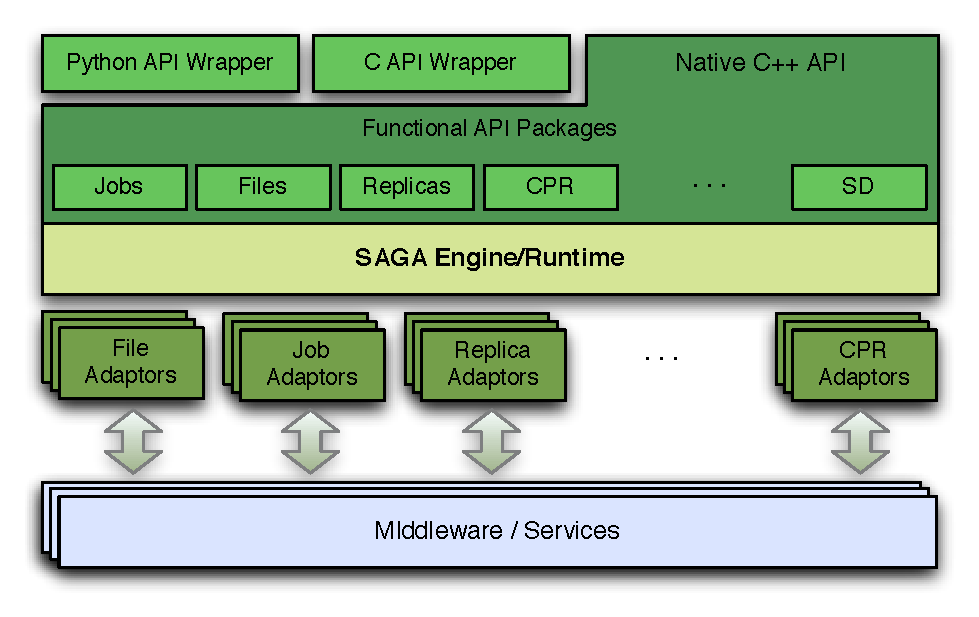
\includegraphics[width=0.40\textwidth]{stci_saga_figures-1.pdf}
 \end{center}
\caption{\small Layered schematic of the different components of the
   SAGA landscape. At the topmost level is the simple integrated API
   which provides the basic functionality for distributed
   computing. Our Big-Job abstraction is built upon this SAGA layer
   using Python API wrapper} \label{Fig:SAGA1}
\end{figure}

\begin{itemize}
\item File package - provides methods for accessing local and remote
 filesystems, browsing directories, moving, copying, and deleting
 files, setting access permissions, as well as zero-copy reading and
 writing
\item Job package - provides methods for describing, submitting,
 monitoring, and controlling local and remote jobs. Many parts of
 this package were derived from the largely adopted
 DRMAA % ~\cite{drmaa_url}                                                                                           
 specification.
\item Stream package - provides methods for authenticated local and
 remote socket connections with hooks to support authorization and
 encryption schemes.
\item Other Packages, such as the RPC (remote procedure call) and Replica
 package
\end{itemize}

In the absence of a formal theoretical taxonomy of distributed
applications, Fig.~\ref{Fig:sagaapps} can act a guide.  Using this
classification system, there are three types of distributed
applications: (i) Applications where local functionality is swapped
for distributed functionality, or where distributed execution modes
are provided.  A simple but illustrative example is an ensemble of an
application that uses distributed resources for bulk submission. Here,
the application remains unchanged and even unaware of its distributed
execution, and the staging, coordination, and management are done by
external tools or agents. Most application in this category are
classified as implicitly distributed.  (ii) Applications that are
naturally decomposable or have multiple components are then aggregated
or coordinated by some unifying or explicit mechanism.  DAG-based
workflows are probably the most common example of applications in this
category.
    % (ii) Applications that are developed using well known patterns,                                                
    % for example MapReduce, which in turn is implemented using                                                      
    % infrastructure independent programming systems such as SAGA;                                                   
Finally, (iii) applications that are developed using frameworks, where
a framework is a generic name for a development tool that supports
specific application characteristics (e.g., hierarchical job
submission), and recurring patterns (e.g., MapReduce, data
parallelism) and system functionality.  SAGA has been used to develop
system-level tools and applications of each of these types.

\begin{figure}[!ht]
  \begin{center}
    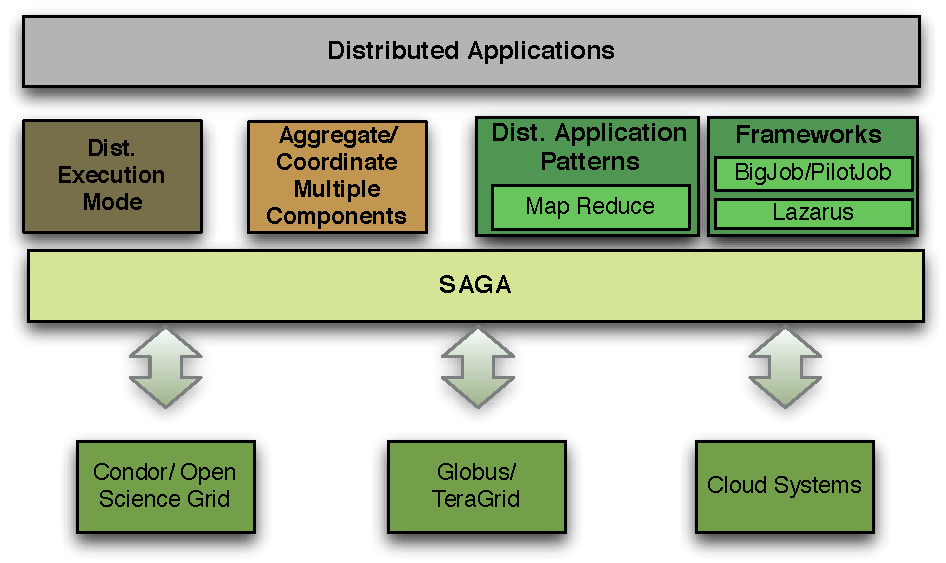
\includegraphics[width=0.45\textwidth]{distributed_applications_saga_figure.pdf}
  \end{center}
  \caption{\small Showing the ways in which
      SAGA can be used to develop distributed applications.
      The different shaded box represent the three different types;
      frameworks in turn can capture either common patterns or common
      application requirements/characteristics. \label{Fig:sagaapps}
      \alnote{Hard to read.} \jhanote{fixed/removed typo. Still hard to read, or better now?}}
\end{figure}

It is important to note that SAGA provides the basic API to
implement distributed functionality required by applications
(typically used directly by the first category of applications),
and is also used to implement higher-level APIs, abstractions, and
frameworks that, in turn, support the development, deployment and
execution of distributed
applications~\cite{gmac09,saga_data_intensive_abstractions}. In
Ref.~\cite{saga_montage} we discussed how SAGA was used to
implement a higher-level API to support workflows. In this paper, 
we will discuss how SAGA can be used to implement runtime
frameworks to support the efficient execution of the distributed
applications.


\Section{Big-Job -- The SAGA-based Pilot-Job} \jhanote{AL}

Pilot-Jobs are a useful abstraction for efficiently executing an ensemble
of batch jobs without the necessity to queue each individual job. A Pilot-Job
is a normal Grid job, which is places into the batch queue of the respective 
Grid resource. Once the batch queue assigned the requested resources to the Pilot-Job,
the Pilot-Job is responsible for managing these and assigning them to so-called Sub-Jobs. 
That way queuing times for Sub-Jobs can be reduced and the predictability for application
scenarios can be increased. 

Pilot-Jobs decouple resource allocation from resource binding and
allow the efficient utilization of resources. By delay the resource
binding decision into the application-level, dynamic usage modes,
e.\,g.\ the load-depended sizing of Sub-Jobs, can be supported.

Big-Job is a SAGA-based Pilot-Job implementation. In contrast to other
Pilot-Job implementations as Condor Glide-In or Falkon, BigJob
natively supports parallel applications (e.g. based on MPI) and works
independent of the underlying Grid infrastructure across different
heterogeneous backend, e.\,g.\ Grids and Cloud, reflecting the
advantage of using a SAGA-based approach. After an overview of the
standard Big-Job implementation for Grid backends, we highlight how
the Big-Job framework was extended to support Condor and Cloud
resources.

\alnote{Old Notes: 
Introduce Big-Job:
 - Describe it, and how it differs from other PilotJobs
 - Outline new usage modes that Big-Job fundamentally supports:
    -- As the basis for scale-out across
    -- As the basis for a framework for runtime optimization
    -- More thought?
Big-Job:
 - Architecture and control flow details
 - Performance Numbers}

\SubSection{Overview}

The following figure gives an overview of the SAGA Big-Job architecture.

\begin{figure}[htbp]
    \centering
    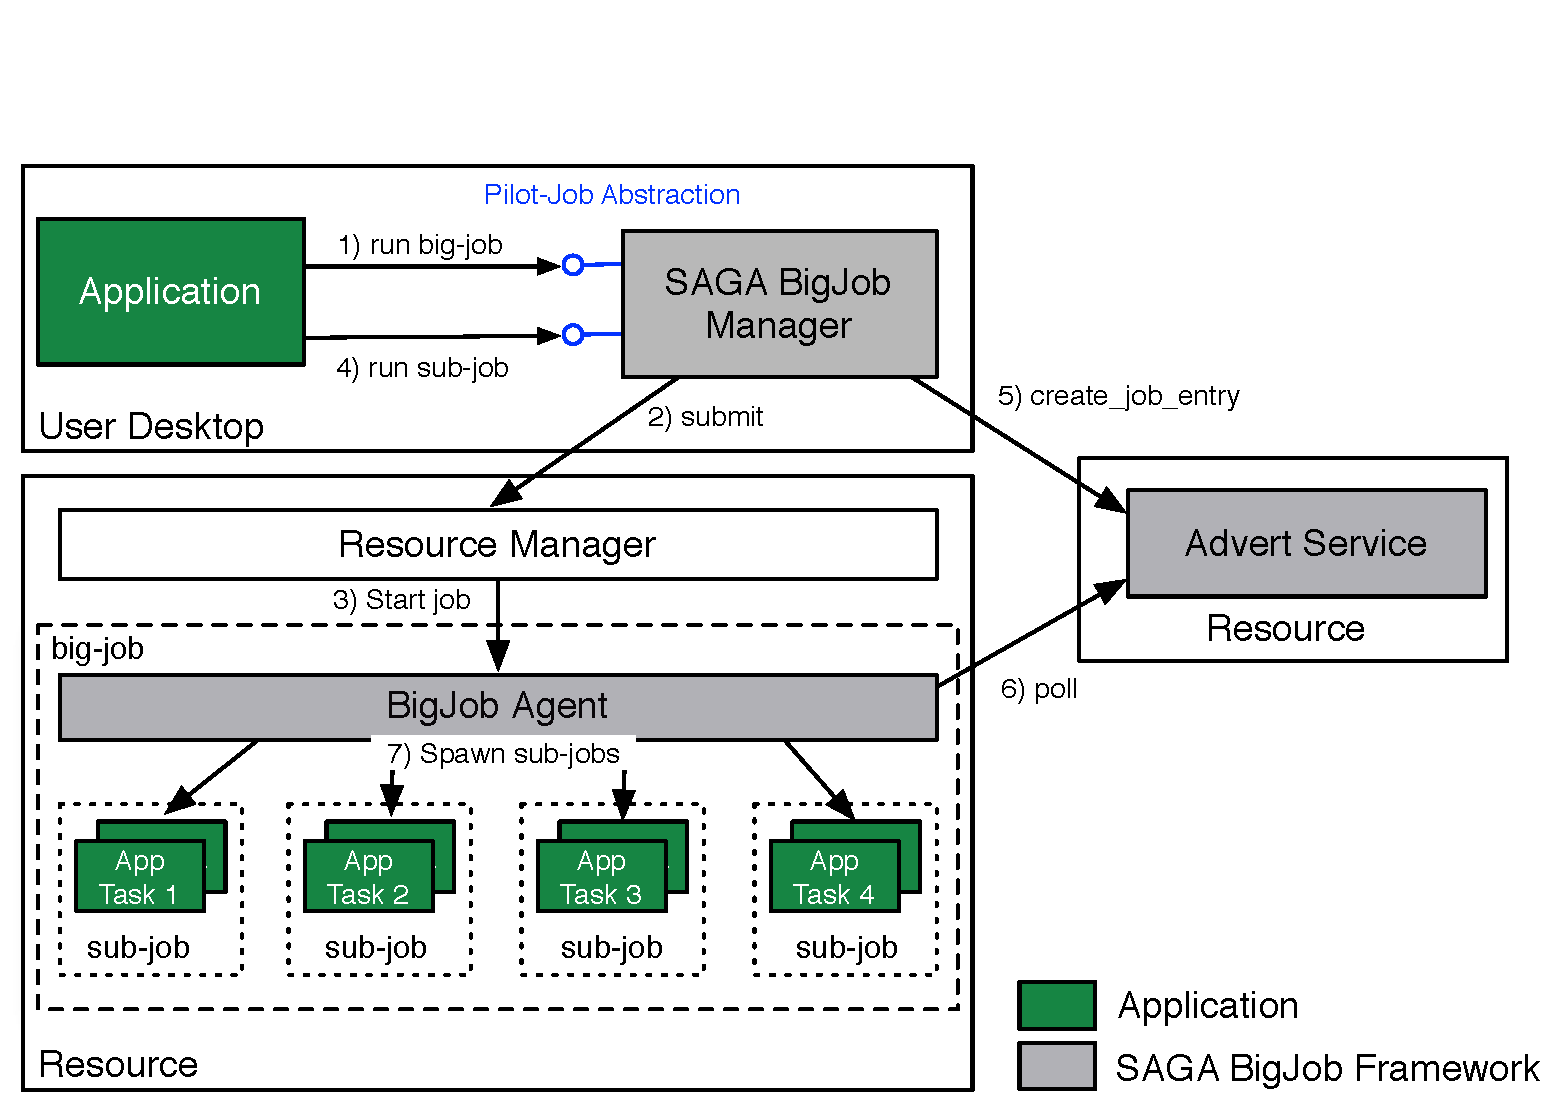
\includegraphics[width=0.45\textwidth]{figures/bigjob}
    \caption{Big-Job Architecture: The core of the framework, the Big-Job-Manager,
     orchestrates a set of Sub-Jobs via a Big-Job-Agents using the SAGA job and file APIs. 
     The Big-Job-Agent is responsible for managing and monitoring sub-jobs on a 
     single machine.}
    \label{fig:figures_bigjob}
\end{figure}

SAGA Big-Job comprises of three components: (i) the Big-Job Manager
that provides the Pilot-Job abstraction and manages the orchestration
and scheduling of Big-Jobs (which in turn allows the management of
both Big-Job objects and subjobs) (ii) the BigJob-Agent that
represents the pilot job and thus, the application-level resource
manager on the respective resource, and (iii) the advert service that
is used for communication between the BigJob Manager and Agent.

Applications can utilize the framework via the \texttt{bigjob} and
\texttt{subjob} classes.  Before running regular jobs, an application
must initialize a \texttt{bigjob} object.  The Big-Job Manager then
queues a Pilot-Job, which actually runs a Big-Job Agent on the
respective resource. For this agent a specified number of resources is
requested. Subsequently, Sub-Jobs can be submitted through the Big-Job
Manager using the jobID of the Big-Job as reference. The Big-Job
Manager ensures that the subjobs are launched onto the correct
resource based upon the specified jobID using the right number of
processes. Communication between the Big-Job Agent and Big-Job Manager
is carried out using the SAGA advert service, a central key/value
store. For each new job, an advert entry is created by the Big-Job
Manager. The agent periodically polls for new jobs. If a new job is
found and resources are available, the job is dispatched, otherwise it
is queued.

\subsection{Big-Job and Condor Glide-in} \jhanote{Lukas}

\jhanote{How bigjob works with Condor Glide-in}

\subsection{Big-Job for Utilizing Cloud Resources} \jhanote{AL}

% espite a standardized interface, big difference on how to obtain meta-data (internal ip etc.)

At the execution level, Clouds differ from Clusters/Grids in at least
a couple of different ways. In Cloud environments, user-level jobs are
not typically exposed to a scheduling system; a user-level job
consists of requesting the instantiation of a Virtual Machine (VM).
Virtual machines are either assigned to the user or not (this is an
important attribute that provides the illusion of infinite resources).
The assignment of job to a VM must be done by the user (or a
middleware layer as Big-Job).  In contrast, user-level jobs on Grids
and clusters are exposed to a scheduling system and are assigned to
execute at a later stage.  Also a description of a Grid/cluster job
typically contains an explicit description of workload; in contrast
for Clouds a user level job typically contains the container
(description of the resource requested) but does not necessarily
contain the workload. In other words, the physical resources are
not provisioned to the workload but are provisioned to the container.
This model is quite similar to resource reservations where you obtain
a ``container'' of resources to which you can later bind jobs
to. Interestingly, at this level of formulation, pilot-jobs attempt to
provide a similar model of resource provisioning as Clouds natively
provide.

Big-Job provides the user an uniform abstraction to Grids and Clouds
independent of any particular Cloud or Grid provider that can be
instantiated dynamically
(Figure~\ref{fig:figures_distributed_pilot_job}).

\begin{figure*}[htbp]
    \centering
        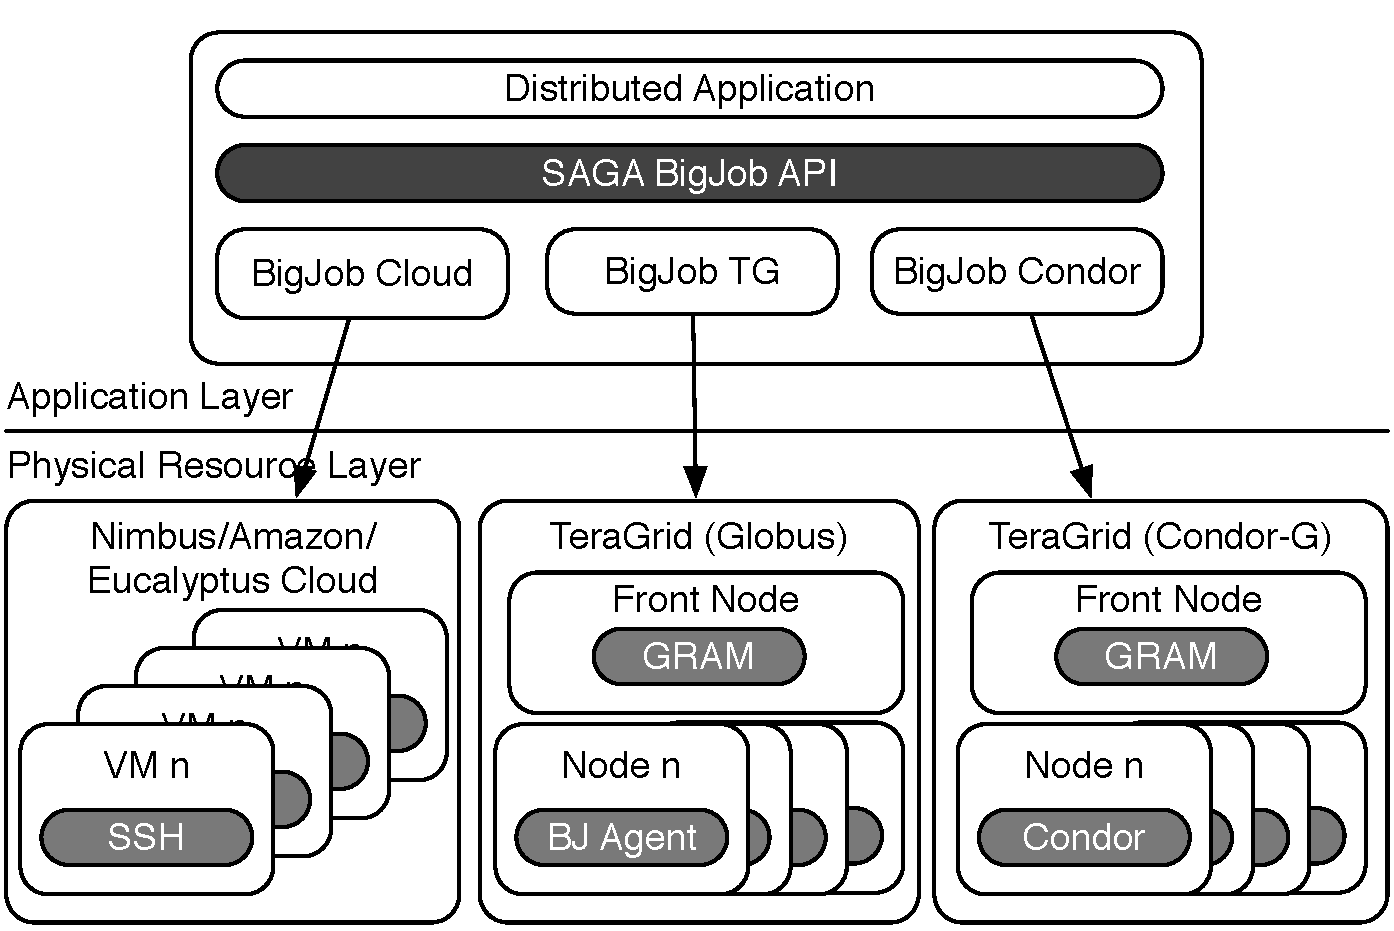
\includegraphics[width=0.7\textwidth]{figures/distributed_pilot_job.pdf}
    \caption{An overview of the SAGA-based Pilot Job}
    \label{fig:figures_distributed_pilot_job}
\end{figure*}

Prior to using the SAGA Cloud Pilot-Job, the user is required to
prepare the virtual machine image for each Cloud that is going to
used. The image should contain the application and possibly the
application data. Once the image is setup, the user can initialize
\texttt{bigjob\_cloud} object referencing the respective Cloud
environment (including the used image).

During the initialization of a Cloud based Big-Job, the implementation
launches the requested number of the specified virtual machine type.
No agent required

While these IaaS Clouds share similar Amazon EC2 style interface, they
tend to expose different semantics and behaviors. Commonly, there a
strong difference in the machine types supported, the management of
metadata and customization possibilities, the image setup procedure,
support for shared file systems, network setup etc. Further
standardization in this area is required.


description of images and instance types different

OCCI

\SubSection{Performance} \jhanote{All}

\alnote{Should we move this section to Usage Model and Analysis?}
\jhanote{I think not. The performance referred to here is that of just
  BigJob startup and dispatch time -- which in principle should be
  independent of any usage mode/scenario. Right?}

Startup Times

Dispatch times

In the following section we show that the SAGA Big-Job abstraction is
suitable for running Pilot-Jobs on different kinds of distributed
infrastructures.

The main overhead when using Big-Job results from the queueing time in Grids respectively the virtual 
machine creation time in Cloud environments. Figure~\ref{fig:performance_setup_time} shows the setup
times observed in our experiments. 
\begin{figure}[htbp]
    \centering
        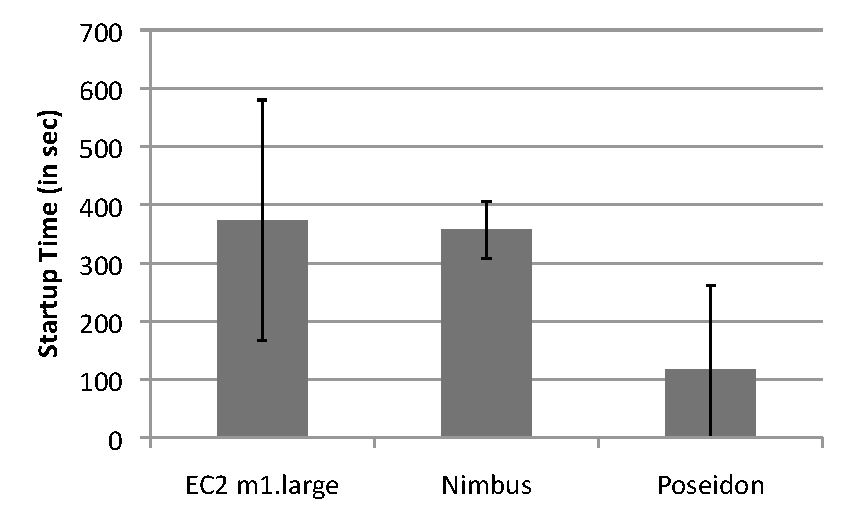
\includegraphics[width=0.45\textwidth]{performance/setup_time_xls.pdf}
    \caption{\textbf{Big-Job Startup Times:} In Grids the startup time
      greatly depends upon the queuing time at the local resource
      manager. However, in our experiments also Clouds showed a high
      fluctuation in the queueing time. \jhanote{Would ``startup''
        time be a better term than ``setup'' time?}}
    \label{fig:performance_setup_time}
\end{figure}


\section{Usage Modes and Analysis}

The aim of this section is not to perform detailed systematic
performance measures and analysis, but to illustrate the various usage
modes the SAGA-based Big-Job can support and how they are supported. We
posit that the performance overheads of Big-Job are small relative to
the duration of the tasks that are typically performed, i.e., order of
seconds compared to tens of minutes and hours.  Needless to say, if
millions of jobs each of short duration were being attempted then the
overheads would be significant.

We discuss two scenarios that are representative of how applications
would typically use multiple distributed infrastructure. We focus our
attention on replica-based MD simulations and define a workload as
\numrep replicas of the HCV model~\cite{}, each replica running for
500 timesteps.  The first scenario involves running all \numrep over
different infrastructure configurations and determining the \tc for
each scenario. We repeat \tc for each configuration \samplenum times.

The second scenario, introduces an upper-bound on the acceptable \tc
(defined as \tmax) -- which is the maximum permissible time to
solution.

Each scenario has several possible specific sub-scenarios, of which we
discuss a few in each.

\subsection{List and explain the resources used in Experiments}

\subsection{Test Application: Scientific Problem Under Study}

\subsubsection*{Resource I: TeraGrid/LONI Cluster (QB)}

\subsubsection*{Resource II: Condor-Pool of LONI Clusters}

\jhanote{This one will require most description -- how the pool is set
up, what features are used etc}

\subsubsection*{Resource III: Cloud Environments}

For our experiments we used different Cloud environments: the Nimbus Science Cloud of the University of Chicago,
the Indiana Eucalyptus Cloud as well as Amazon EC2.


\subsection{Scenario I: \tc for Workload for Different Resource Configurations}

\subsubsection{\tc for single Resource Usage}

In the first example, a given workload -- a NAMD simulation consisting
of xxx atoms -- was run for 500 timesteps at different
infrastructures. For this experiment the Charm++~\cite{871085} version
of NAMD was used; Charm++ is in this case just a wrapper layer around
MPI (so as to address dependencies).

In most cases the TeraGrid and LONI machines QB and Poseidon outperform the Cloud resources. 
However, there are scenarios when Cloud resources were
able to outperform HPC resources, e.\,g.\ a single replica run required more than 5\,sec less
on the largest available EC2 instance with 68.4\,GB of memory and 8\,virtual cores than on Poseidon
or QB. 

\begin{figure}[htbp]
    \centering
    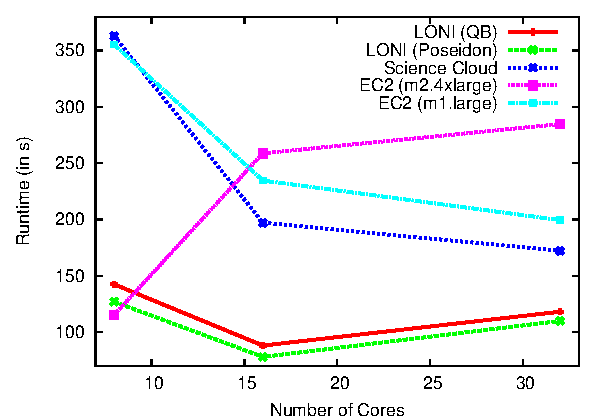
\includegraphics[width=0.45\textwidth]{performance/namd_run.pdf}
    \caption{\textbf{NAMD Runtimes on Different Resource Types: } The graph shows that 
             native HPC resource generally outperform Cloud resources in particular when
             running applications across multiple nodes. However, the new high memory eight 
             core EC2 instance type was able to complete a replica run faster than QB or Poseidon.}
    \label{fig:performance_namd_run}
\end{figure}

On the HPC resources \tc decreased when using up to 16\,cores. With more cores a slight increase can
be observed. In most EC2 and Nimbus scenarios the \tc decreased with the number of instances and cores
used. When using the largest EC2 instance and increase of \tc can be observed. These behavior is particularly
caused by the slow interconnects between these instances. Generally those interconnects are heavily oversubscribed
in particular in the EC2 environment causing this massive slowdown. In the following experiments we 
will use replica jobs with the size of 8 cores as basis. In this scenario the cost/performance
ratio is particularly in Clouds optimal. 

\subsubsection{\tc for Collective Resource Utilization}

In this scenario we used the Big-Job abstraction to run replicas across different types of
infrastructures. In this experiment the LONI cluster Poseidon and the Nimbus Cloud at the University
of Chicago are used. At the beginning of the experiment a particular set of Pilot-Jobs is started
in each environment. Once a Pilot-Job becomes active, the application assigns replica to 
this job. We measure \tc for different sizes of Pilot-Jobs. Figure~\ref{fig:performance_8replica_scenario_poseidon_nimbus}
shows the results.

\begin{figure}[htbp]
    \centering
        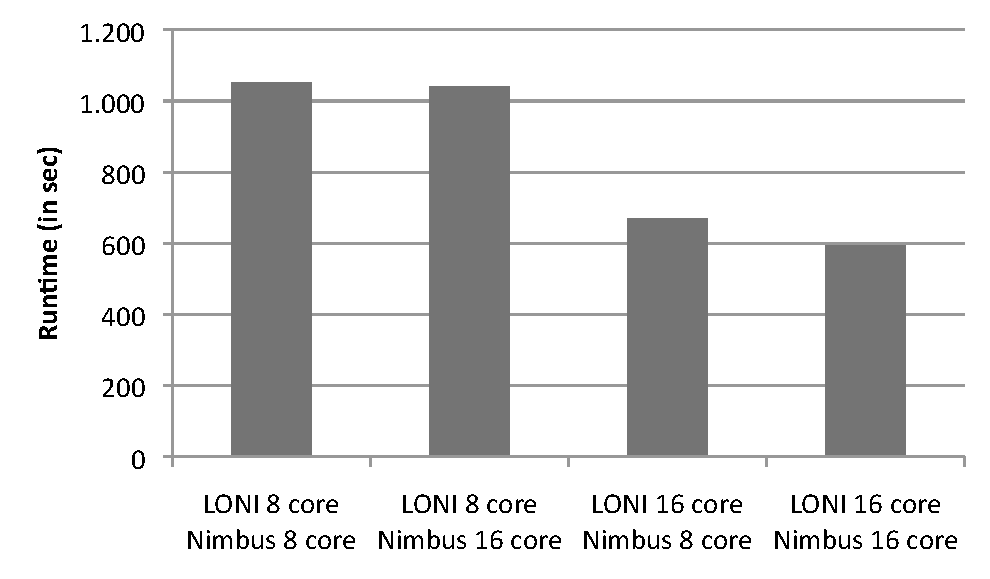
\includegraphics[width=0.45\textwidth]{performance/8replica_scenario_poseidon_nimbus}
    \caption{\textbf{Collective Usage of Cloud and Grid Resources: }  The experiments showed that if the LONI resource
             Poseidon has only a light load, the benefits of using additional Cloud resources are very low. Increasing
             the size of the Nimbus Pilot-Job only resulted in modest improvements of \tc. 
             However, when using more Poseidon resources \tc could be reduced by more than 6 minutes.}
    \label{fig:performance_8replica_scenario_poseidon_nimbus}
\end{figure}


\begin{itemize}
\item Resource I and III:
\item Resource II and III:
\item Resource I, II and III:
\end{itemize}


If resources in the Grid environment are instantly available it is usually not reasonable to start
additional Cloud resources. However, Clouds provide a very predictable startup times. Thus,
it is possible to  Nevertheless,
the performance can be highly variable.

\subsection{Scenario II: Investigation of the Distribution of Workload for Maximum Allowed
  Time to Solution} 

Given that Clouds provide the illusion of infinite capacity, or at
least queue wait-times are non-existent, it is likely that often most
sub-jobs will end up on the Cloud infrastructure.  Thus, in Scenario
II, the resource assignment algorithm we use is as follows: We submit
tasks to non-Cloud resources first. Periodically the progress of the
scenario is monitored. If not sufficient jobs have finished
when time equal to $T_{X}$ has elapsed,
%(defined as: \tmax - 2 average \tc on all Clouds)  
than we move the workload to utilize Clouds.  The
underlying basis is that Clouds have an explicit cost associated with
them and if jobs can be completed on the the TG and Condor pool while
preserving the performance constraints, we opt for such a
solution. However, if queue loads prevent the performance requirements
being met, we move the jobs to a Cloud-resource, which we have shown
has less fluctuation in \tc of the workload.

For this experiment we integrated a progress manager that implements
the described algorithm into the replica application.
The user has the possibility to specify a maximum runtime and a check interval.
At the beginning of each check interval the progress manager compares the number 
of jobs done with the total number of jobs and estimates the total 
number of jobs that can be completed within the requested timeframe. If the total
number of jobs is higher than this estimate, the progress monitor instantiates
another Big-Job object request additional cloud resources for a single replica. 
In this scenario, each time an intermediate target is not met four additional 
Nimbus VMs sufficient for running another eight core replica are instantiated.
Table~\ref{tab:app_deadline} summarizes the results.

\begin{table}[ht]
    \centering
	\begin{tabular}{|l|l|l|}
	\hline
    Result & \#\,Events &Average \tc \\ \hline
	No VM started &6 &7.8\,min\\ \hline
	1 VMs started &1 &36.4\,min\\ \hline
	2 VMs started &1 &47.3\,min\\ \hline
	3 VMs started &2 &44.2\,min\\ \hline
	\end{tabular}
	\caption{Usage of Cloud Pilot-Jobs to Ensure Deadline \label{tab:app_deadline}}
\end{table}

In the investigated scenario, we configured a maximum runtime of
45\,minutes and a progress check interval of 4 minutes. We repeated
the same experiment 10\,times at different times of the day. In 6 out
of 10\,cases the scenario completed in about 8\,minutes. In the other
cases additional VMs had to be started to finish the application
within the specified deadline. In two cases 3\,Pilot-Jobs each with 8
cores had to be started to meet the application deadline. In one case
a single Pilot-Job was sufficient. In a single case the deadline was
missed solely due to the fact that not sufficient Cloud resources have
been available. \jhanote{Put note to say something about fluctuations
  on Grids/Clusters}.

\alnote{Old notes: This scenario in particular shows how Big-Jobs can
  be dynamically created based on runtime decisions.  Based on current
  trends: will we finish or not.  Poseidon Big-Job becomes available
  after 100 sec 1 replica finishes after 150 sec After 1/4 check
  whether some resources should be started: - 1 Big-Job on Nimbus with
  4 VM - increase VMs linearly if jobs done don't catch - if we caught
  up, we backup}



\Section{Conclusion}
various abstractions for IaaS currently
various standardization efforts: OCCI, Cloud Consortium, ISO

We plan to extend this work in two important directions. The first is
the use of a more sophisticated coordination mechanism -- that
supports asynchronous task coordination (e.g., Comet). In this paper,
we have focussed on replica simulations, but not on replica-exchange
simulations -- which involve coordination between the different tasks
and intelligence in their placements.  It will be very interesting to
note the performance gains that accrue as a result of such
asynchronous coordination on production infrastructure for the
replica-exchange problems. Also, having established the basic
infrastructure to submit tasks to and manage multiple, heterogenous
resources using a simple, single interface, an important second
extension of this work is to use more sophisticated task-placement
decisions or resource utilization decision making.

\bibliographystyle{IEEEtran}
\bibliography{saga,literatur}
\end{document}
